\documentclass[a4paper]{arrowhead}

\usepackage[yyyymmdd]{datetime}
\usepackage{etoolbox}
\usepackage[utf8]{inputenc}
\usepackage{multirow}
\usepackage{hyperref}

\renewcommand{\dateseparator}{-}

\setlength{\parskip}{1em}

%% Special references
\newcommand{\fref}[1]{{\textcolor{ArrowheadBlue}{\hyperref[sec:functions:#1]{#1}}}}
\newcommand{\mref}[1]{{\textcolor{ArrowheadPurple}{\hyperref[sec:model:#1]{#1}}}}
\newcommand{\pdef}[1]{{\textcolor{ArrowheadGrey}{#1\label{sec:model:primitives:#1}\label{sec:model:primitives:#1s}\label{sec:model:primitives:#1es}}}}
\newcommand{\pref}[1]{{\textcolor{ArrowheadGrey}{\hyperref[sec:model:primitives:#1]{#1}}}}

\newrobustcmd\fsubsection[3]{
  \addtocounter{subsection}{1}
  \addcontentsline{toc}{subsection}{\protect\numberline{\thesubsection}function \textcolor{ArrowheadBlue}{#1}}
  \renewcommand*{\do}[1]{\rref{##1},\ }
  \subsection*{
    \thesubsection\quad
    operation
    \textcolor{ArrowheadBlue}{#1}
    (\notblank{#2}{\mref{#2}}{})
    \notblank{#3}{: \mref{#3}}{}
  }
  \label{sec:functions:#1}
}
\newrobustcmd\msubsection[2]{
  \addtocounter{subsection}{1}
  \addcontentsline{toc}{subsection}{\protect\numberline{\thesubsection}#1 \textcolor{ArrowheadPurple}{#2}}
  \subsection*{\thesubsection\quad#1 \textcolor{ArrowheadPurple}{#2}}
  \label{sec:model:#2} \label{sec:model:#2s} \label{sec:model:#2es}
}

\begin{document}

%% Arrowhead Document Properties
\ArrowheadTitle{Orchestrator Core System}
\ArrowheadType{System Description}
\ArrowheadTypeShort{SysD}
\ArrowheadVersion{4.6.0}
\ArrowheadDate{\today}
\ArrowheadAuthor{Rajmund Bocsi}
\ArrowheadStatus{RELEASE}
\ArrowheadContact{rbocsi@aitia.ai}
\ArrowheadFooter{\href{www.arrowhead.eu}{www.arrowhead.eu}}
\ArrowheadSetup
%%

%% Front Page
\begin{center}
  \vspace*{1cm}
  \huge{\arrowtitle}

  \vspace*{0.2cm}
  \LARGE{\arrowtype}
  \vspace*{1cm}

  %\Large{Service ID: \textit{"\arrowid"}}
  \vspace*{\fill}

  % Front Page Image
  %\includegraphics{figures/TODO}

  \vspace*{1cm}
  \vspace*{\fill}

  % Front Page Abstract
  \begin{abstract}
    This document provides system description for the \textbf{Orchestrator Core System}.
  \end{abstract}

  \vspace*{1cm}

%   \scriptsize
%   \begin{tabularx}{\textwidth}{l X}
%     \raisebox{-0.5\height}{
\includegraphics[width=2cm]{figures/artemis_logo}} & {ARTEMIS Innovation Pilot Project: Arrowhead\newline
%     THEME [SP1-JTI-ARTEMIS-2012-AIPP4 SP1-JTI-ARTEMIS-2012-AIPP6]\newline
%     [Production and Energy System Automation Intelligent-Built environment and urban infrastructure for sustainable and friendly cities]}
%   \end{tabularx}
%   \vspace*{-0.2cm}
 \end{center}

\newpage
%%

%% Table of Contents
\tableofcontents
\newpage
%%

\section{Overview}
\label{sec:overview}
\color{black}
This document describes the Orchestrator Core System, which exists to find matching providers for the consumer's specification within an Eclipse Arrowhead Local Cloud (LC) and in other Arrowhead clouds by collaborating with other Core Systems. This can be achieved by using stored matching rules or applying a more dynamic strategy using the Service Registry Core System. This mandatory Core System provides the data storage functionality for the information related to matching rules and optionally provider reservation.

The rest of this document is organized as follows.
In Section \ref{sec:prior_art}, we reference major prior art capabilities
of the system.
In Section \ref{sec:use}, we describe the intended usage of the system.
In Section \ref{sec:properties}, we describe fundamental properties
provided by the system.
In Section \ref{sec:delimitations}, we describe delimitations of capabilities
of the system.
In Section \ref{sec:services}, we describe the abstract service
operations produced by the system.
In Section \ref{sec:security}, we describe the security capabilities
of the system.

\subsection{Significant Prior Art}
\label{sec:prior_art}

The strong development on cloud technology and various requirements for digitisation and automation has led to the concept of Local Clouds (LC).

\textit{"The concept takes the view that specific geographically local automation tasks should be encapsulated and protected."} \cite{jerker2017localclouds}

An orchestration system is a central component in any Service-Oriented Architecture (SOA). In applications the use of SOA for a massive distributed System of Systems requires orchestration. It is utilised to dynamically allow the re-use of existing services and systems in order to create new services and functionality. 

\subsection{How This System Is Meant to Be Used}
\label{sec:use}

Orchestration is a mandatory core system of Eclipse Arrowhead LC and is responsible for finding and pairing service consumers and providers. 

An application that want to consume a service should ask the Orchestrator to find one or more accessible providers that meet the necessary requirements (including Quality-of-Service requirements). The Orchestrator returns the information (address, port, context path, tokens) that the application needs to consume the specified service.

\subsection{System functionalities and properties}
\label{sec:properties}

\subsubsection {Functional properties of the system}
Orchestrator solves the following needs to fulfill the requirements of orchestration.

\begin{itemize}
    \item Enables the application and other core systems to find the appropriate providers to consume their services.
    \item Enables the Workflow Choreographer core system to find appropriate providers for its executors to consume the services.
    \item Enables the Plant Description Engine core system to create and remove flexible matching rules.
    \item Enables the Gatekeeper core system to handle provider reservations in the name of an other cloud.
\end{itemize}

\subsubsection {Non functional properties of the system}
The Orchestrator implements certain authentication capabilities, meaning that Orchestrator makes decision whether a given system has right to use its services (i.e. only the Workflow Choreographer can orchestrate providers for some other systems).

\subsubsection {Data stored by the system}
In order to achieve the mentioned functionalities, Orchestrator is capable to store the information set described by figure \ref{fig:information_overview}.

\begin{figure}[h!]
  \centering
  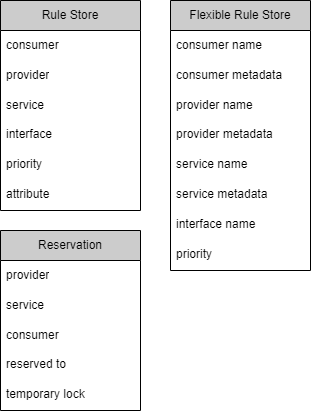
\includegraphics[width=8cm]{figures/orchestrator_data_overview.png}
  \caption{
    Overview of data stored by Orchestrator Core System.
  }
  \label{fig:information_overview}
\end{figure}

\subsection{Important Delimitations}
\label{sec:delimitations}

While Orchestrator Core System is capable of using two types of matching rules (fix rules where every pairing is referencing a consumer and a provider instance, or flexible rules where both consumer and provider can be described with their names and/or their settings), can't use both simultaneously. Administrators have to choose between the two modes when deploying the system.

Also, the Orchestrator can't work alone. It needs a Service Registry Core System and a Authorization Core System to operate. To enable inter-cloud orchestration, it also needs at least a running Gatekeeper Core System and depending on networking a Gateway Core System, too. To enable Quality-of-Service requirement matching, a QoS Monitor Core System is needed.

\newpage

\section{Services produced}
\label{sec:services}

\msubsection{service}{echo}
The purpose of this service is to test the system availability. The service is offered for both application and core systems. 

\msubsection{service}{orchestration-service}
The purpose of this service is to get access information for providers that provides the required service and meets the additional requirements. The service is offered for both application and core systems. 

\msubsection{service}{orchestration-service-by-proxy}
The purpose of this service is to get access information for providers that provides the required service and meets the additional requirements. The main difference between this service and the previous one that here the consumer of the service is not the requester system. The service is offered only for the Workflow Choreographer Core System. 

\msubsection{service}{orchestration-service-by-id}
With this service a consumer can get access information for all its necessary services based on the top priority stored matching rules. The service is offered for both application and core systems.

\msubsection{service}{orchestration-create-flexible-store-rules}
The purpose of this service is to create flexible matching rules. The service is offered only for the Plant Description Engine Core System.

\msubsection{service}{orchestration-remove-flexible-store-rule}
The purpose of this service is to remove a flexible matching rule. The service is offered only for the Plant Description Engine Core System.

\msubsection{service}{orchestration-clean-flexible-store}
The purpose of this service is to remove all flexible matching rules. The service is offered only for the Plant Description Engine Core System.

\msubsection{service}{orchestration-qos-enabled}
The purpose of this service is to tell the requester whether the Orchestrator can handle Quality-of-Service requirements or not. The service is offered only for Gatekeeper Core System.

\msubsection{service}{orchestration-qos-reservations}
The purpose of this service is to return all active provider reservations. The service is offered only for Gatekeeper Core System. 

\msubsection{service}{orchestration-qos-temporary-lock}
The purpose of this service is to lock a set of providers temporarily. The service is offered only for Gatekeeper Core System. 

\msubsection{service}{orchestration-qos-confirm-reservation}
The purpose of this service is to confirm a temporary provider reservation. All related not confirmed reservation are released. The service is offered only for Gatekeeper Core System. 

\newpage

\section{Security}
\label{sec:security}

The security of Eclipse Arrowhead - and therefore the security of Orchestrator  - is relying on X.509 certificate trust chains. The Arrowhead trust chain consists of three level:
\begin{itemize}
    \item Master certificate: \texttt{arrowhead.eu}
    \item Cloud certificate: \texttt {my-cloud.my-company.arrowhead.eu}
    \item Client certificate: \texttt{my-client.my-cloud.my-company.arrowhead.eu}
\end{itemize}

For Arrowhead certificate profile see \url{https://github.com/eclipse-arrowhead/documentation}

\newpage

\bibliographystyle{IEEEtran}
\bibliography{bibliography}

\newpage

\section{Revision History}
\subsection{Amendments}

\noindent\begin{tabularx}{\textwidth}{| p{1cm} | p{3cm} | p{2cm} | X | p{4cm} |} \hline
\rowcolor{gray!33} No. & Date & Version & Subject of Amendments & Author \\ \hline

1 & YYYY-MM-DD & \arrowversion & & Xxx Yyy \\ \hline
\end{tabularx}

\subsection{Quality Assurance}

\noindent\begin{tabularx}{\textwidth}{| p{1cm} | p{3cm} | p{2cm} | X |} \hline
\rowcolor{gray!33} No. & Date & Version & Approved by \\ \hline

1 & YYYY-MM-DD & \arrowversion  &  \\ \hline

\end{tabularx}

\end{document}